\subsection{Covariate Shift Intensity and OOD Detection}
We first assess the accuracy of the \gls{ood} detectors across the types and intensities of shifts. This was achieved by computing \gls{ba} scores for each shift and shift intensity, for the \gls{ood} detectors associated with the highest accuracy on the organic \gls{ood} data. The results are shown in \Cref{fig:accuracy}. 
\begin{figure*}
    \centering
    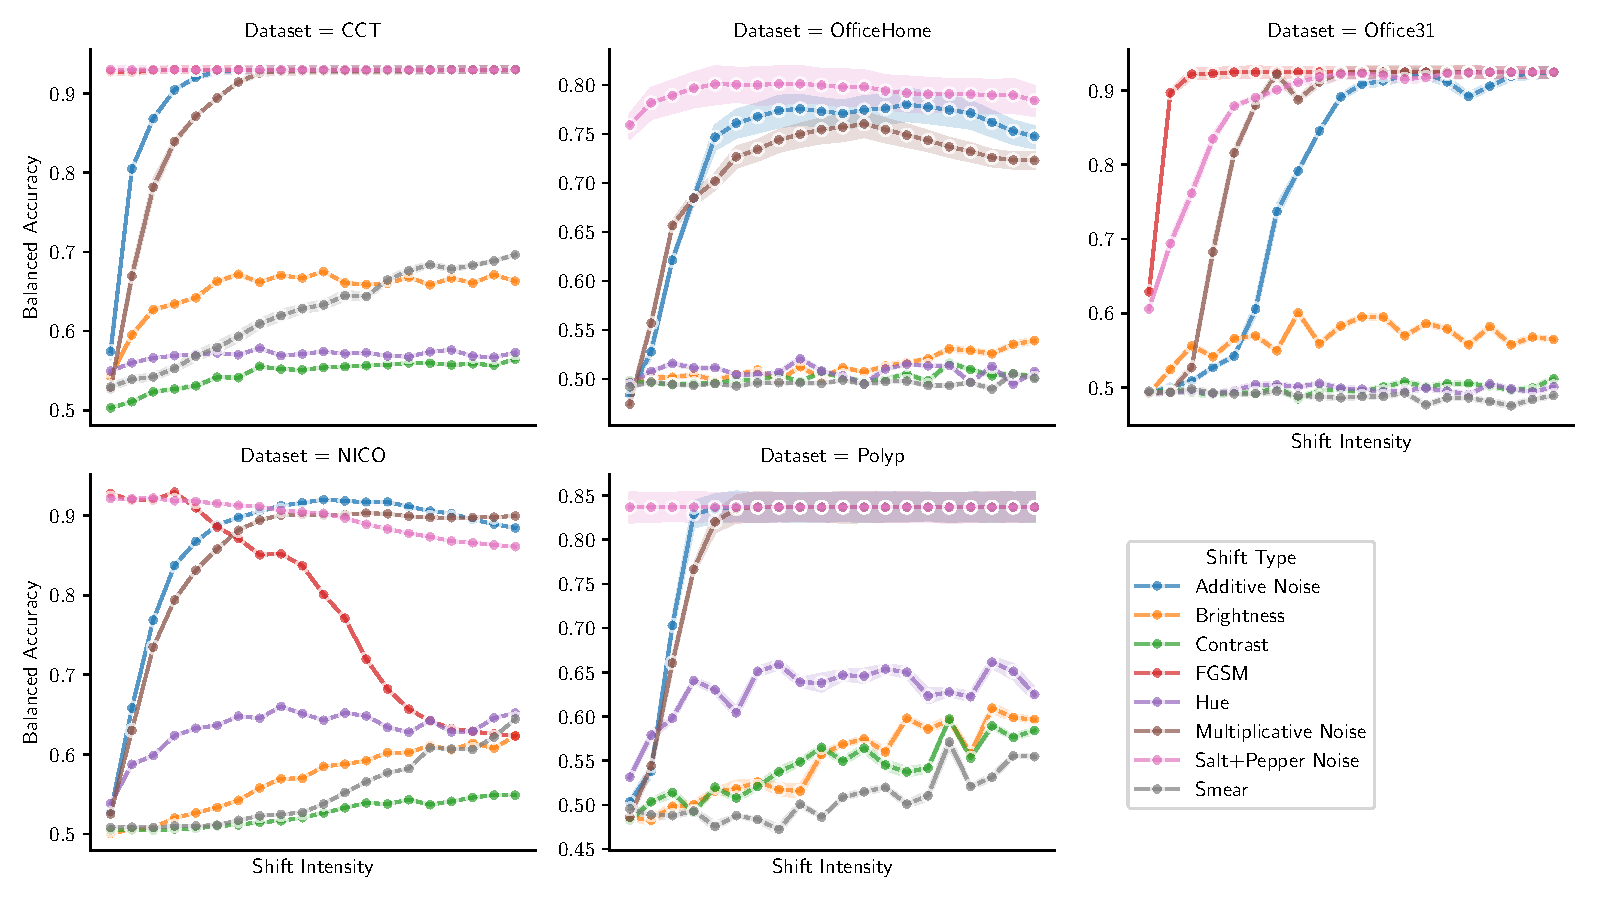
\includegraphics[width=\linewidth]{figures/shift_intensity_vs_ba.pdf}
    \caption{Shift intensity \(\alpha\) vs \gls{ood} detector \gls{ba} across shifts for the best performing \gls{ood} detectors for each dataset.}
    \label{fig:accuracy}
\end{figure*}

Overall, we observe that certain shifts are often associated with fairly high \gls{ood} detector accuracy while others may be associated with lower accuracy. Notably, shifts in contrast, brightness, distortions, and hue are generally less readily detected than the different types of noise. We conjecture that this difference may be attributed to the fact that noise may often break low-level features~\cite{noise_robustness, corruption_robustness}, and that they therefore manifest more distinctly in the \gls{ood} detector features. 

The results also show that shifts of greater intensity are generally associated with higher \gls{ood} detector accuracy. This can be attributed to the fact that data that have undergone shifts of greater intensity are generally more distinct from the training data, and therefore that \gls{ood} detectors more readily separate them. There is, however, one notable exception to this, namely for FGSM shifts on the NICO dataset. Here, higher intensities are associated with lower accuracies. While we do not observe this phenomenon on any of the other datasets, we conjecture that this is attributable to the specific effects of adversarial attacks on data. Adversarial attacks yield data that is visually near-\gls{ind}, but which nevertheless are beyond the manifold of the training data~\cite{adversarial_bugs_features}. 



 and more generally the infeasibility of curating data sets with sufficient coverage of real-world characteristics\cite{data_work}, particularly those that manifest infrequently, such as rare diseases\cite{medical_low_sample} or otherwise rare events\cite{av_low_sample}. 


 However, these results are often misleading\cite{testing_ml, testing_ml2, benchmarking_validity}, as testing datasets do not typically account for the full scope of the diversity of data that can be encountered in real-world settings. Indeed, as these test-sets are often sampled from the training data, e.g., in hold-out evaluation or cross-validation, they are characterized by the same latent biases in the data collection as the training datasets themselves. \Glspl{dnn} trained on ImageNet, for instance, often fail to generalize to ImageNet-like datasets\cite{imagenet_gen}, and likewise with CIFAR10/100\cite{cifar_gen}, precisely because these new datasets are characterized by a moderately dissimilar set of biases. 


This is known as \textit{generalization failure}, and can be largely attributed to the prevalence of \gls{iid} violations in training datasets and the underspecified regime in which \glspl{dnn} are trained~\cite{damour2020underspecification, shortcut_learning}. 

\Gls{erm}, the basis for supervised learning, can only guarantee generalization for predictors of bounded complexity\cite{deep_learning_book, vapnik_statistical_learning}. \Glspl{dnn}, on the other hand, are characterized by extremely high complexity\cite{randomlabels}. The apparent ability of \Glspl{dnn} to generalize beyond the training data is therefore dependent on sufficient regularization, either explicitly through methods such as batch normalization~\cite{batchnorm}, data augmentation~\cite{generalization_datamod}, regularizing loss terms~\cite{l2_reg}, etc.\cite{regularization_survey}, or implicitly through the design of \Gls{dnn} architectures\cite{implicit_bias}. This permits generalization beyond the empirical distribution of the training data, typically manifesting as high performance on benchmarks and hold-out evaluations. 


\section{Accuracy Estimation}
In the previous section, we showed that there is frequently a strong relationship between the generalization gap associated with a particular shift and the rate at which these shifts are detected by \gls{ood} detectors. We exploit this relationship in order to approximate the accuracy attained by the given \gls{dnn}. This can be achieved by fitting a regression model that maps a given \gls{ood} detection rate to an estimated network accuracy. We compute this detection rate for a batch of data through the following estimator:
\begin{equation}
    DR = \frac{1}{|X|} \sum_{x \in X} d(x)
\end{equation}
where \(d\) is the \gls{ood} detector and \(X\) is the set of inputs in a given sequence. Note that the data with which we train the model assumes that the data sequence for which we compute \(DR\) is composed of \gls{iid} data relative to the nature of a given covariate shift. In real-world scenarios, a given sequence of data may be subject to different types of covariate shift. Suppose that the observed sequence \(X\) is composed of samples drawn from multiple distinct covariate shifts \(\{S_i\}\), each occurring with a relative frequency \(w_i\) such that \(\sum_i w_i = 1\). The accuracy of the model on this mixture can, asymptotically, be expressed as the weighted mean of its accuracies under the constituent shifts:
\begin{equation}
    A_{\text{mix}} = \sum_i w_i A_i,
\end{equation}
where \(A_i\) denotes the accuracy of the model under shift \(S_i\). For the proposed estimation framework to generalize to sequences composed of multiple different types and intensities of covariate shifts, the predictor of accuracy ---namely, the detection rate --- must exhibit the same composability property. 


Specifically, the detection rate measured on a mixed sequence should equal the weighted mean of the detection rates observed under its constituent shifts:
\begin{equation}
    DR_{\text{mix}} = \sum_i w_i DR_i.
\end{equation}
This requirement constrains the form of the mapping between detection rate and accuracy. If the regression function \(f(\cdot)\) relating \(DR\) to \(A\) is nonlinear, then
\[
f(DR_{\text{mix}}) \neq \sum_i w_i f(DR_i),
\]
and estimation errors will arise whenever the incoming data stream contains heterogeneous shifts. To preserve composability under mixtures of shift types, the mapping must therefore be \textbf{linear (or affine)}:
\begin{equation}
    \hat{A} = \alpha \, DR + \beta,
\end{equation}
where \(\alpha\) and \(\beta\) are obtained through least-squares fitting on data with known accuracies and measured detection rates. This linear formulation ensures that when several covariate shifts co-occur in a given sequence, the predicted accuracy of the mixture equals the weighted mean of the predicted accuracies of its components. 
